%
% $RCSfile: template_method.tex,v $
%
% Copyright (C) 2002-2008. Christian Heller.
%
% Permission is granted to copy, distribute and/or modify this document
% under the terms of the GNU Free Documentation License, Version 1.1 or
% any later version published by the Free Software Foundation; with no
% Invariant Sections, with no Front-Cover Texts and with no Back-Cover
% Texts. A copy of the license is included in the section entitled
% "GNU Free Documentation License".
%
% http://www.cybop.net
% - Cybernetics Oriented Programming -
%
% http://www.resmedicinae.org
% - Information in Medicine -
%
% Version: $Revision: 1.1 $ $Date: 2008-08-19 20:41:09 $ $Author: christian $
% Authors: Christian Heller <christian.heller@tuxtax.de>
%

\subsubsection{Template Method}
\label{template_method_heading}
\index{Template Method Pattern}
\index{Hook Method Pattern}

The \emph{Template Method} pattern \cite{gamma1995}, also called
\emph{Hook Method}, is an abstract definition of the \emph{Skeleton} of an
algorithm. The implementation of one or more steps of that algorithm is
delegated to a sub class (figure \ref{templatemethod_figure}).

\begin{figure}[ht]
    \begin{center}
        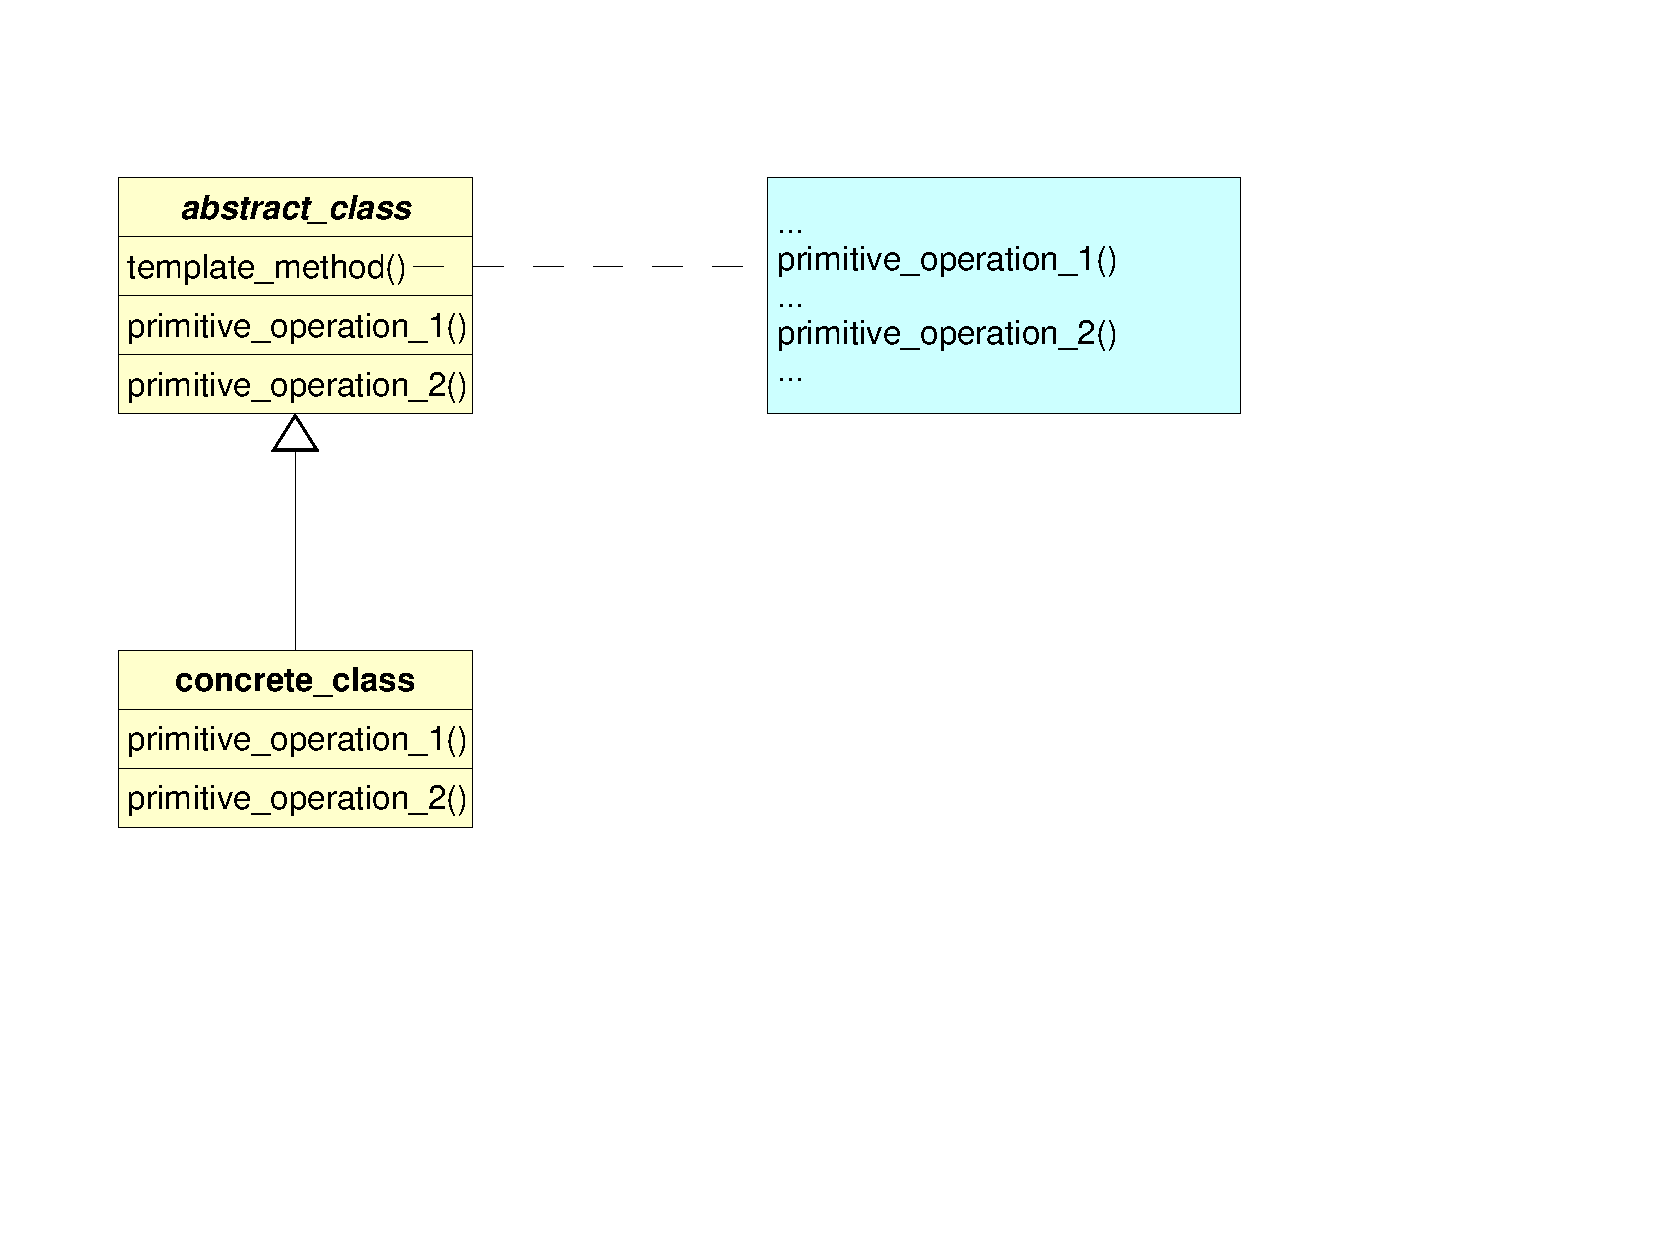
\includegraphics[scale=0.3,angle=-90]{graphic/templatemethod.pdf}
        \caption{Template Method Pattern}
        \label{templatemethod_figure}
    \end{center}
\end{figure}

The idea of algorithm (method) templates was taken over in the design of the
new language described in chapter \ref{cybernetics_oriented_language_heading}.
The single template parts, however, are not inherited but implemented in
\emph{part} templates referenced by their corresponding \emph{whole} template,
which is actually more similar to the previously described \emph{Whole-Part}
pattern (section \ref{design_heading}).
